\documentclass[11pt]{article}
\usepackage{amsfonts}
\usepackage{amssymb}
\usepackage{amsmath}
\usepackage{amsthm}
\usepackage{titlesec}
\usepackage[hidelinks]{hyperref}
\usepackage{enumitem}
\usepackage{geometry}
\usepackage[round]{natbib}
\usepackage{booktabs}
\usepackage{tikz}
\usetikzlibrary{snakes}
\usepackage{rotating}
\usepackage{array}



\setlength{\parskip}{0.75em}
\let\oldemptyset\emptyset \let\emptyset\varnothing 

\newtheorem{definition}{Definition}

\title{Project P-15:\\Approaches to Computational Stem Completion}
\author{Frederik Glitzner\\fr725212@dal.ca\\B00910841}
\date{\today}

\begin{document}
\maketitle

\begin{abstract}
    Stemming is natural language processing technique, applied for example in information retrieval, text compression and text similarity measuring. The output of a stemming algorithm, however, is not trivially invertible. This leads to the Stem Completion Problem, which is the computational reconstruction of the original words given a vector of stems. This project aims to study the Porter Stemmer applied to English language texts and the corresponding stemming statistics and to design algorithms and solutions to the Stem Completion Problem by discussing a variety of methods of both traditional and machine learning methods.
\end{abstract}

\tableofcontents
\listoffigures
\listoftables



\section{Problem Statement}

\subsection{Introduction}

Stemming is a widely used natural language processing technique reducing words to their word stem, which is not necessarily its root. A stemming algorithm takes any word consisting of a sequence of letters as its input, follows fixed rules for conversion and returns a new word.
As such, it is impossible to invert the algorithm and restore the removed suffix. This project aims to design and discuss multiple approaches to reconstructing the original word from the stem using both traditional and machine learning methods.

\begin{table}[!ht]
    \centering
    \title{\Large Desired algorithm behavior\\}
    \begin{tabular}{p{0.08\linewidth}p{0.25\linewidth}p{0.18\linewidth}p{0.2\linewidth}}
        Given: & Algorithm $A$ so that & $A(($"engineering"$))$ &$=$ ("engin") \\
        Goal: & $\hat{A}$ so that & $\hat{A}(($"engin"$))$ &$=$ ("engineering") \\
    \end{tabular}
    \caption{Visual example of the desired algorithm behavior}
\end{table}

\subsection{Formal Definition of the Problem}

\begin{definition}[Stem Completion Problem]
    Let $\sum = \{a,b,...,z\}$ be the alphabet of lowercase latin letters and $w\in(\sum^*\setminus{I})^n$ be a vector of words in this alphabet without infinite sequences $I$. A suffix-removing stemming algorithm $A$ will, for each word $w_i\in w$, add, modify or remove letters of $w_i$ and return a new word $w_i'=A(w_i)$ called stem so that $\vert w_i' \vert\leq \vert w_i \vert$ and $w_i'\cap w_i \neq \emptyset$. Note that not necessarily $w_i'\subseteq w_i$. Then the Stem Completion Problem is to determine the original vector of words $w$ given the vector of words $w'$. We restrict this problem further by reducing the input space $\sum^*\setminus{I}$ to the language $L$ consisting of words used in English literature.
\end{definition}

\subsection{Main Challenge}

By definition of the stem completion problem, we have 
$$A : W \rightarrow W'\mbox{; } w \mapsto w' $$
with, for $w_i\in w$, $w_i' = A(w_i)$, $\vert w_i' \vert\leq \vert w \vert$,
so in general $\vert W' \vert\leq \vert W \vert$ and actually $\vert W' \vert < \vert W \vert$. Therefore $A$ cannot be surjective, so there cannot exist an inverse function $A^{-1}$ of $A$. Therefore, an approximation algorithm $\hat{A}$ of $A^{-1}$ must be found in order to solve the Stem Completion Problem.

The practical challenge of finding an approximation is the dynamic behavior of words in natural language depending on syntactic and semantic context. Syntactically, suffixes can be induced for example by personal pronouns, e.g. "she reads" instead "she read", or by grammatical rules, e.g. "she is reading" instead of "she is read", although the intended meaning of the words "(to) read", "reads" and "reading" is equivalent. However, sentence constructs can be arbitrarily complex, not just depending on the previous word, inducing complex word behavior dependencies. See for example the sentence "she, who has read many books in her life, would, given the opportunity, have bought this library". In this sentence it can be seen how the phrase "she would have bought" can be fragmented through injecected subordinal clauses. Semantically, the same stem can correspond to multiple distinct word meanings. For example, the word "Usingeer", which could be a name, corresponds to the stem "using", which is a potential word itself with not only a completely different meaning but also a completely different part of speech function. Better examples of this will be available after completion of the stem analysis phase of this project.

\subsection{Motivation}

Apart from the theoretical challenge, there are multiple motivations to study the reconstruction of stems. Stemming is used in information retrieval, especially in search queries where the aggregation of words with the same meaning but different spelling, for example due to grammatical rules, is essential \citep{UyarStemming}. 

\begin{table}[!ht]
    \centering
    \title{\Large Example IR Query: \textit{"Connection"}}
    \begin{tabular}{p{0.4\linewidth}p{0.4\linewidth}}
        \textbf{Document Content} & \textbf{Stemmed Word} \citep{porterstemmer} \\
        ...connect... & connect \\
        ...connects... & connect \\
        ...connected... & connect \\
        ...connecting... & connect \\
        ...connection... & connect \\
        ...connections... & connect \\
    \end{tabular}
    \caption{Example grouping of words by their stem}
\end{table}

Given these methods in information retrival, the indexed documents and other forms of textual data need to be stemmed, but the original form of the documents must be maintained for the query response. However, if a stem completion algorithm would provide a reliable responses with a high accuracy, it would be possible to eliminate the original form and reduce the amount of data stored and maintained to the reduced stemmed version of the data. Moreover, this would provide a computationally efficient method for text compression while maintaining the ability to reproduce the original form of the document.
In the broader context of science, stem completion plays a large role in psychological, specifically implicit memory, and medical research. \cite{pmid26321987}, for example, outlines experiments about the effect of priming, that is the exposure to a stimulus without conscious guidance, on this task and finds that significant correlations can be measured. \cite{pmid17065885} studies the subconscious memory performance of patients under the influence of anesthesia using the task of stem completion to study deviations in patient response before and after surgery. Although a computational solution is not directly relevant to this research, it would provide new opportunities for research at the intersection of human and computer performance and behavior, for example the study of bias in data-driven algorithms against human bias \citep{TIGGEMANN200473}.
More philosophically, this idea resulted from the question asking how many books a computer must process given a method of computational learning to accurately reflect the conventions and grammatical rules of natural language. 
Lastly, the Stem Completion Problem is a prime example of a task where traditional methods in natural language processing are not sufficient and more advanced methods are needed.



\section{Relevant Work and Possible Approaches}

\subsection{Previous Work}

The only resource to be found after an extensive search for papers on computational stem completion or stem inversion is by \cite{Feinerer2010} who provides a proof that the problem corresponding to his definition is NP-hard, shown via a polynomial-time reduction from the set cover problem. Furthermore, \cite{Feinerer2010} designs an experiment to test the accuracy of a simple stem inverter. His inversion algorithm $A$ takes a vector of stems $w$ and a corpus of words $C$. \cite{Feinerer2010} then defines five heuristics that $A$ can be based on: 
\[ A(w_j)=
\begin{cases} 
    \mbox{Prevalent: }c\in C \mbox{ such that} & \mbox{max}_{i=1,...,n}\vert c_i\vert = c \\
    \mbox{First: }c\in C \mbox{ such that} & c_1 = c \mbox{ (first in the dictionary)} \\
    \mbox{Shortest: }c\in C \mbox{ such that} & \mbox{min}_{i=1,...,n}\vert \mbox{char}c_i\vert = c \\
    \mbox{Longest: }c\in C \mbox{ such that} & \mbox{max}_{i=1,...,n}\vert \mbox{char}c_i\vert = c \\
    \mbox{Random: }c\in C \mbox{ such that} & c_i = c \mbox{ with } i = \mbox{random}(1,...,n)\\
\end{cases}
\]
Note that $n$ denotes the total number of completions for a given term.

In simple terms, given a stem $w_j$, $A_{\mbox{heuristic}}$ with heuristic $\in \{$Prevalent, First, Shortest, Longest, Random$\}$ searches the dictionary for words that match the stem and, if successful, returns one of them, with the choice depending on the heuristic. 

\cite{Feinerer2010} then evaluates the accuracy of each $A_{\mbox{heuristic}}$ using the Reuters-21578 data set \citep{ReutersDataset} based on three measures: Reconstruction (here called stem completion), Text Clustering (application of heuristic to text clustering) and Sentiment Analysis (comparison of sentiment analysis results on stemmed words against completed words as a measure of sentimental similarity). The results show that in Reconstruction, the heuristics Prevalent, First and Shortest outperform Random and Longest. In Text Clustering, the heurstic Prevalent outperforms First and Random, which outperform Shortest, which outperform None (no heuristic), which performs better than Longest. Lastly, in Sentiment Analysis, Prevalent and First outperform Shortest, which outperforms Longest, which outperforms Random. Overall, in the reconstruction experiment, None performs with an average 43\% accuracy and the best heuristic, Shortest, performs with an average 67.46\% accuracy. His algorithm is used in the function \textit{stemCompletion} in the R package \textit{tm} \citep{stemcompletionpackage}.

This project aims to reconstruct and extend the experiments conducted by \cite{Feinerer2010}, conduct a deeper analysis of stems on a different dataset and discuss other approaches to stem completion.

\subsection{Data Pipeline}

First, with the implementation of the popular Porter Stemmer as described by \cite{porterstemmer}, a clear image of how this stemming algorithm works will be outlined. Roughly, the algorithm groups the characters of the given input word into single or successive vowels and consontants and then applies a sequence of three clearly defined transformation steps based on both the characters and the vowel-consonant structure of the word. The output is a word with length at most the length of the input word that intersects with the input word but does not need to be a subset of the input word. 

To conduct statistical analysis on stems and as a basis for further experiments, a dataset consisting of a variety of texts from Project \cite{gutenberg}, specifically books and novels, will be assembled. Standard text processing methods will be applied to the data, such as the removal of empty lines, unrecognized characters and punctuation. The data from different sources will be merged into a single data pool and shuffled in a sentence structure preserving way in order to reduce source-bias. This makes one part of the dataset; the other part starts with a copy of this data pool, applies the Porter Stemmer to each word and saves the stemmed data. The resulting dataset for the naive implementation will be a sequence of words both in their unstemmed and in their stemmed version. Later in the experiment's data pipeline, these data pools will be split into a training and a testing set. 

\subsection{Naive Approach}

The naive solution to the Stem Completion Problem for a given stem $w'$ and the fact that $A$ is injective but not surjective is to generate all possible inputs $w$ so that $A(w)=w'$, thereby aiming for an algorithm $\hat{A}$ so that $\hat{A}(w')=\{w\in L \vert A(w=w')\}$. This requires full knowledge of $L$, however, it is impossible to limit the input space $L$ to a finite number of words. \cite{wordlength} finds that the average word length in common English language is around 4.6 characters, so even when assuming a range of $1\leq \vert w\vert \leq 15$, the combinatorial approach generates an input space of size $\sum_{i=1}^{15}26^{i}-s_i$ for $26$ letters in the alphabet and accounting for $s_i$ combinations of letters that do not make sense phonetically in the English language. 

Our hypothesis is, however, that the input space of common English language can be bounded, that is, the number of distinct words decrease over time when processing large amounts of common English language data. Therefore, the dataset as described above will be generated by analysis of a text corpus, generating a mapping $M:W'\rightarrow W^n$ by determining $w'=A(w)$ for each seen distinct word $w$ in the corpus and $n$ being the maximum number of processed words for a given stem, and approximating the input space by $L=W$. For the experiment, the dataset will be split into a training and a testing dataset and only the training dataset will be used to generate the mapping $M$.

The intended behavior of $\hat{A}$ is to take a list of stems $w'$ as input and return a list of lists of seen words $w_i$ so that for each $w_i$, $A(w_i)=w'_i$. A potential evaluation method for $\hat{A}$ is to feed in the stems of the testing dataset as input $w'$ and measure how many of the correct words are present in the output $\hat{A}(w')$.

\subsection{Selective Approach}

The idea behind the selective approach is to reduce the output of the naive algorithm $\hat{A}$ to a list of words rather than a list of lists of words by selecting one word for each stem using heuristics. Using heuristics corresponds to the approach that \cite{Feinerer2010} took in solving the Stem Completion Problem.

We will evaluate the accuracy of different heuristics again by feeding in the stems of the testing dataset as input $w'$ and measure how many of the correct words are present in the output $\hat{A}(w')$ for each heuristic. It will be interesting to see whether the results of this slightly different implementation and a different dataset will match the results found by \cite{Feinerer2010}.

\subsection{Using Natural Language Models}

The selective approach is unlikely to perform well. Statistically, some heuristics may perform okay, but given the simplicity, the accuracy must be bounded by the combinatorics of the problem. Therefore, assuming English language sentences as input, the next logical step in designing an algorithm $\hat{A}$ is to not view the stem in isolation, but rather extend the view to a neighborhood of that stem in the given input vector through a language model, that is, a probabilistic model estimating the probability of an arbitrary natural language sentence \citep{vlado}.

One approach is to use pure language modeling. In a brute-force solution, the output of the naive approach could be combined combinatorially by generating every possible sentence given the output of the naive algorithm and then fed into a language model trained on English language sentences, predicting the probability of each given sentence. The output of the algorithm would then be the sentence with the highest probability given the language model. Alteratively, the algorithm could be designed more sequentially by choosing the first stem completion of the sentence using a heuristic and choosing every subsequent completion with a language model given the previous completions. For this, the n-gram model could be chosen for example. 

Another approach is through part-of-speech tagging. The possible procedures are similar to the ones above, but more abstract. In part-of-speech tagging, words are divided into classes depending on their function in a sentence \citep{nlpbook}.
Using a part-of-speech tagger, each word in the output of the naive approach could be tagged and then either all order-preserving permutations could be generated and evaluated by a probabilistic model trained on part-of-speech abstracted sentence structures, or the choice of completions could be sequentially by starting with a completion corresponding to a likely sentence start part-of-speech tag and choosing the next most likely completion sequentially. 

In both approaches and both procedures, although especially the sequential procedure, it is expected to quickly run into difficulties when given longer, more complex sentences and additionally, these approaches are only likely to show improvement over the selective approach when given a stemmed real English sentence as input and not when the desired stem completions are unrelated in context. As a potential improvement of the sequential, one-directional procedure, a bidirectional selection could be tried using bidirectional part-of-speech combinatorics, with the drawback of increased computational complexity.


\subsection{Advanced Machine Learning Methods}

As outlined above, the Stem Completion Problem has both an unconstrained input and an unconstrained solution space and rule-based systems are unlikely to perform well. Thus, a data-driven approach could be more effective, and especially knowing off the problems of variable context and bidirectional dependencies as explained in the problem statement, modern advanced machine learning techniques are well-suited for further experimentation. 

As an advancement of the n-gram model mentioned above, which incorporates the context of a fixed number of previous words or stems to calculate a probability for the given stem being a certain word, a Long Short-Term Memory model \citep{lstm} trained on stems and stem completions would provide additional flexibility for the context and take into account not just the shallow close context, but also important bits of context from more distant parts of the input, making a more promising candidate model for complex sentence structures like the example given in the problem statement. The Long Short-Term Memory model is a recurrent neural network architecture paired with gradient-based learning algorithm for a constant error flow through internal flow of special units \citep{lstm}. Through a combination of memory cell blocks, the model becomes a probabilistic unidirectional structure and was originally applied to time lag problems such as embedded Reber grammar learning and noisy signal processing.

The most recent paradigm-changing paper in this field was published by \cite{transformerOrig} and outlines a new model called Transfomer for bidirectional processing and probabilistic reasoning for arbitrary input lengths through self-attention. 
The original Transformer has an Encoder-Decoder architecture with Multi-Head Attention layers playing the most novel role. These layers can be described as mapping a query vector and key-value vector pairs to an output vector, which is the weighted sum of the values given the keys and query over several attention layers in parallel. The core motivations for self-attention are reduced computational complexity per layer compared to other neural network architectures, the amount of parallelization possible during the computation and finally the ability to learn long-range dependencies for applications in sequence transduction tasks \citep{transformerOrig}.
The hypothesis is that by combining multiple layers of self-attention, each layer can learn a different subspace of the problem and contribute to a final classification. The original paper applies a Transformer model to the problem of machine translation.
In one experiment, the model learns English-to-German language translation and outperforms all previously published models at a fraction of the training cost of any other competitive model. An experiment for English-to-French translation shows similar results \citep{transformerOrig}. Transformers have has since proven successful in a many tasks and variations and are used by BERT \citep{bert}, which stands for Bidirectional Encoder Representations from Transformers and is a technique for natural language processing pre-training developed by Google, and the GPT models \citep{gpt}, which stands for Generative Pre-trained Transformer and is an autoregressive language model developed by OpenAI producing text with the goal of being non-distinguishable from high-quality human text.

This project also aims to dive deeper into how Long Short-Term Memory and attention-based Transformer models work and how they could be applied to this problem.


\section{Project Plan}


The followings tasks are planned to be carried out in the 5 calendar weeks 45-49: 

\begin{table}[!ht]
\centering
\begin{tabular}{p{0.01\linewidth}p{0.44\linewidth}>{\centering\arraybackslash\hspace{0pt}}p{0.215\linewidth}>{\centering\arraybackslash\hspace{0pt}}p{0.22\linewidth}}
& \textbf{Task} & \textbf{Time Est. (\%)} & \textbf{Report Est. (\%)}\\
\hline
0 & Gather dataset and implement data pipeline & 6 & 6 \\
1 & Study and implement the Porter Stemmer & 9 & 14 \\
2 & Conduct statistical analysis of stems & 14 & 13 \\
& - Growth of distinct stems &  &  \\
& - Distribution of stem frequencies &  &  \\
& - Unique stems against unique words &  &  \\
3 & Write up theoretical challenge & 7 & 8 \\
& - Problem Statement &  &  \\
& - Context and Bidirectional Dependency &  &  \\
4 & Design, implement and evaluate the naive solution & 9 & 13 \\
5 & Improve the naive solution through Heuristics & 5 & 10 \\
6 & Design methodology to improve naive solution through language models & 10 & 9 \\
7 & Provide overview of how advanced machine learning methods could be applied to this problem & 15 & 15 \\
& - N-Gram Model &  &  \\
& - Long short-term memory &  &  \\
& - Transformer &  &  \\
8 & Outline motivation for this project & 5 & 4 \\
& - Information Retrieval / Compression &  &  \\
& - Reference to the social sciences &  &  \\
9 & Write the rest of the report & 20 & 8 \\
\end{tabular}
\caption{List of remaining tasks with estimated proportion of time commitment and estimated proportion of final report length}
\end{table}



\begin{figure}[!ht]
\centering
\resizebox{0.5\columnwidth}{!}{%
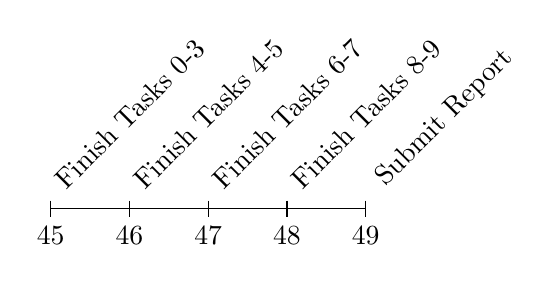
\begin{tikzpicture}
    % draw horizontal line   
    \draw (-5,0) -- (-1,0);
    
    % draw vertical lines
    \foreach \x in {-5,-4,-3,-2, -1}
    \draw (\x cm,3pt) -- (\x cm,-3pt);
    
    % draw nodes
    \draw (-5,0) node[below=3pt] {$ 45 $} node[above=3pt] {$  $};
    \draw (-4,0) node[below=3pt] {$ 46 $} node[above=3pt] {$\begin{turn}{45} Finish Tasks 0-3 \end{turn}$};
    \draw (-3,0) node[below=3pt] {$ 47 $} node[above=3pt] {$\begin{turn}{45} Finish Tasks 4-5 \end{turn}$};
    \draw (-2,0) node[below=3pt] {$ 48 $} node[above=3pt] {$\begin{turn}{45} Finish Tasks 6-7 \end{turn} $};
    \draw (-1,0) node[below=3pt] {$ 49 $} node[above=3pt] {$\begin{turn}{45} Finish Tasks 8-9 \end{turn}$};
    \draw (0,0) node[below=3pt] {$  $} node[above=3pt] {$\begin{turn}{45} Submit Report \end{turn}$};
\end{tikzpicture}%
}
\caption{Milestone overview with distribution of remaining tasks on calendar weeks}
\end{figure}


\clearpage
\bibliographystyle{plainnat}
\bibliography{refs}

    
\end{document}